\documentclass{article}

\usepackage{scribe}

\setseriestitle{Probabilistic Machine Learning and Inference}
\setscribecode{1}
\setauthname{Gurpreet Singh}
\setinstrname{Piyush Rai}
\setheaddate{Decemenber 1, 2017}
\settitle{Introduction to Probabilistic Machine Learning}

\begin{document}
\makeheader

Generally, the data we observe has some noise. Sometimes, we need to model this error or uncertainty explicitly. Often, we also need probabilistic predictions (fraudulent transaction). For this we need probabilistic modelling of our problem. \br

There could also be uncertainties in the estimated model parameters, or the predictions itself can be uncertain. To model these uncertainties, we require a probabilitic approach.

\begin{ssection}{Probabilistic Modelling of Data}

	We generally assume the data points to be independent of each other, and dependent on only unknown paramters (say $\vtheta$) \et{i.e.} we ssume data $\vX = \set{\vx^1, \vx^2 \dots \vx^N}$ to be generated from a probabilistic model with an unknown parameters $\vtheta$

	\begin{align*}
		\vx^1, \vx^2 \dots \vx^N	\qsim	\prob{\vX \pipe \vtheta}
	\end{align*}

	Since the points are assumed to be independent, we can aslo say

	\begin{align*}
		\prob{\vX \pipe \vtheta}	\eq	\prod_{n = 1}^N \prob{\vx^n \pipe \vtheta}
	\end{align*}

	\begin{ssubsection}{Representing Probabilitic Models}

		We generally use a simplistic ``plate-notation'' graphical model to represent probabilistic models.

		\begin{figure}[h!]
			\centering
			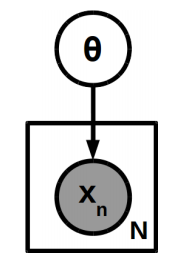
\includegraphics[width=0.1\textwidth]{includes/scribe01/plate-graphical-model.png}
			\caption{Plate-Notation Graphical Model}
			\label{fig:plate-model}
		\end{figure}

		In the plate-notation, the shaded nodes represent known or observed values, whereas unshaded nodes represent unknown or learned variables, and the arrows show dependency. \br

		In the example in figure \ref{fig:plate-model}, $\vX = \set{\vx^1, \vx^2 \dots \vx^N}$ is known, and $\vtheta$ is learned. Also, $\vX$ is dependent on $\vtheta$. \br

		\note{Partially shaded nodes represent partially observed or missing values. For example, in semi-supervised learning} \br

		Any node that we are uncertain about (can also be the observed nodes) is modelled using a probability distribution and these nodes become the random variables of the model. \br

		The full model is specified via a joint probability distribution over all random variables.

	\end{ssubsection}

	\begin{ssubsection}{Parameter Estimation}

		Specification of probabilistic models requires two key ingredients -- Likelihood and Prior \br

		\begin{definition}[Likelihood Function]
			This is the observation model that specifies how data is generated. This measures the data fit w.r.t. to the given parameters $\vtheta$ and is represented by the conditional property $\prob{\vX \pipe \vtheta}$
		\end{definition}

		\begin{definition}
			Prior Distribution specifies how likely different parameter values are a priori. This also acts as a regularizer to the model and is represented by the prior probability $\prob{\vtheta}$
		\end{definition}

		For parameter estimation, we have two methods, point estimate or Bayesian Inference. \br

		A single point estimate is represented as the simple maximization problem

		\begin{align*}
			\widehat{\vtheta}_{MLE}	\eq	\argmax{\vtheta} \prob{\vX \pipe \vtheta}
		\end{align*}

		This is known as the Maximum Likelihood Estimate (MLE). We can also have a regularized version, by maximising the posterior of the parameter, instead of the Likelihood Function. This is known as the Maximum-a-Posteriori (MAP) Estimate. \br

		\begin{align*}
			\widehat{\vtheta}_{MLE}	&\eq	\argmax{\vtheta} \prob{\vtheta \pipe \vX} \\
									&\eq	\argmax{\vtheta} \prob{\vX \pipe \vtheta} \prob{\vtheta}
		\end{align*}
		
		However, we cannot measure the uncertainty in the estimated parameter value. Hence, we use Bayesian Inference. We can estimate the full posterior distribution over $\vtheta$ to get the uncertainty.

		\begin{align*}
			\prob{\vtheta \pipe \vX}	\eq	\frac{\prob{\vX \pipe \vtheta} \prob{\vtheta}}{\prob{\vX}}
		\end{align*}

		We can also use Bayesian Inference in an online setting, where the old posterior can act as the new prior. Hence, our belief about $\vtheta$ keeps getting updated as wee see more and more data.

	\end{ssubsection}

\end{ssection}

\begin{ssection}{Generative Modelling}

	Generative models are typically probabilistic, specifying a joint probability distribution over observation and target (label) values. A conditional distribution can be formed from a generative model through Bayes' rule. \br

	Each data point $\vx^n$ is associated with a latent variable $\vz^n$, which is essentially a compact representation or encoding of the data point. For example, in case of Gaussian Mixture Models, the latent variable is the cluster assignment. The latent variables can also be used to infer missing data or \et{relevance} of a data point (hence generative). \br

	Generative models are used in many problems (mostly unsupervised) such as GMM, Probabilistic PCA, Deep Generative Models, etc.
	
\end{ssection}

\end{document}
